\section{Existing System}
Currently, majority of the ride-sharing coordination is done manually via phone calls, messaging app, or a social media platform. These old approaches are disjointed and inefficient and lead to communication failure, absence of transparency, and safety\cite{chaudhry2018}. As an example, the riders and drivers find it hard to make schedules or confirm actions of the rides because there is no centralized system to handle the booking, confirming, and cancellations. Also, the users are not able to trace their past rides, sums spent, and revenues effectively. The other major drawback is that there is lack of emergency management leaving the riders unprotected in case of accidents or suspicious cases. Administrators also do not have real-time monitoring dashboard and tools and it is hard to monitor the work of the platform, identify improper behavior, or to be accountable. In this way, the existing model is not organized, not trustworthy, and cannot effectively meet the increasing need of the safe and community-focused ride-sharing models.

\section{Proposed Solution}
The new Wheel Share system will bring a monolithic, automated and convenient system that ensures that all ride-sharing functions are incorporated within one mobile and web application. Wheel Share uses Flutter because it is a cross-platform platform or stacks and Supabase because it has real-time background distribution assurance to provide its customers with smoother functionality, high safety, and engaging access of its applications. Riders, Drivers, and Admins of the system have role-based dashboards to make the system more user-friendly and secure. Users will be able to post rides, find the available ones by city, address or date, and deal with the driver. Drive through an in-built dashboard is capable of sending offers, accepting rides and managing their overall earnings\cite{acheampong2021}. The system will also have building trust ratings and reviews under its system, emergency alert mechanisms to release the safety of the system and Administration Module to oversee the system, manage and monitor emergency activities. It also has a search and filtering tool of rides and transactions to enhance effectiveness. The suggested solution is projected to lessen the communication limitations, improve the levels of trust and transparency, and offer a safe and effective setting of shared mobility. 


\section{Functional Requirements}

\textbf{User Authentication: }
\begin{enumerate}[label=\roman*.]
 The system allows individuals to create and log in using email and password credentials through Supabase Auth, and manage the sessions and change passwords and personal profiles. 
    
\end{enumerate}

\textbf{Ride Management: }
\begin{enumerate}[label=\roman*.]
The drivers are offered with option of posting the rides with destination by address of the city and date. Riders can locate rides according to the various filters and invite to join any available rides. Obstacles that have been posted can be edited and erased when the need arises. 
    
\end{enumerate}

\textbf{Offer Management: }
\begin{enumerate}[label=\roman*.]
The drivers who seek to take up rides may send offers and these offers may be rejected or accepted by the riders. This has contributed to this being flexible and in control by the two experiencing ride coordination. 
\end{enumerate}

\textbf{Ratings and Reviews: }
\begin{enumerate}[label=\roman*.]
Following a ride, the users can do a review and comment upon each other. Such ratings help in maintaining reliability, improve quality of service and foster transparency. 
\end{enumerate}

\textbf{Emergency Feature: }
\begin{enumerate}[label=\roman*.]
The system also has irritating alarm feature that allows people (riders or drivers) to call the admin instantly in case of emergency to have the required action taken in time and remain safe. 
\end{enumerate}
\textbf{Admin Module:  }
\begin{enumerate}[label=\roman*.]
The admin will be able to handle the total user activities, ride management and the rating issue, delete the unnecessary user account and also track the emergencies. Adequate accountability may also be done by admins who can address reports and system logs.  
\end{enumerate}

\section{Non-Functional Requirements}

\begin{enumerate}[label=\roman*.]
    \item \textbf{User Interface:} The Wheel Share application provides an easy to use interface in Flutter version based on Web, Android and iOS applications giving users of any ability level ease in navigating the functionality. 
    
    \item \textbf{Security:} The platform uses a high security future and Supabase Row-Level Security (RLS) to protect the credentials of the users, the rides, and the payment details. 

\end{enumerate}

\subsection{Performance:} Basic functions like posting of rides, searching and offer response should be done within 2-3 seconds and this renders the users with quick and interactive interactions. 
\begin{enumerate}[label=\roman*.]
    \item \textbf{Reliability:} The system will be built to guarantee 99.9% uptime, which is ensured by automatic data backups to avoid losses in the system in the event of failure or crashes. 
    \item \textbf{Scalability:} The system will be built to guarantee 99.9% uptime, which is ensured by automatic data backups to avoid losses in the system in the event of failure or crashes. 
    \item \textbf{Compatibility:  } The app can support the recent models of the mobile operating system and web browsers which proves to be device-friendly.  
\end{enumerate}

\subsection{Audit and Compliance: }
\begin{enumerate}[label=\roman*.]
All big operations such as ride posts, offers, approvals and emergency alerts are real-time logged to provide transparency, accountability and auditing. 
\end{enumerate}





\section{Use Cases}
A UML use case diagram are graphical illustrations that show how the users  interact with what the system is able to do. When applied to Wheel Share, these diagrams show the interaction between Riders, Drivers, and the Admins and different modules of the platform. The Rider is able to modify and create rides, transfer and receive offers and rate the rides. The Driver has an opportunity to find rides, earns, and accept offers to work. Admin is responsible of the running of all system activities such as monitoring of users and tracking of the ride, as well as dealing with emergency alerts. The diagrams allow developers to gain an overview of the scope of the system and simplify how the system functions were viewed by a user. They are also used as a basis in the definition of test cases, refinement of requirements and also in ensuring that the final implementation is in line with the expectations of the stakeholders. 

\subsection{Use Case Diagram of WheelShare System}

\noindent
This use case diagram illustrates the interaction between the main actors of the WheelShare system, including Rider, Driver, and Admin. It shows the core functionalities such as ride posting, ride searching, sending and accepting offers, and triggering emergency alerts. The diagram also represents administrative operations like user management, ride monitoring, and performance evaluation. Overall, it provides a high-level view of how different users interact with the system to support safe and efficient ride sharing.

\begin{figure}[H]
    \centering
    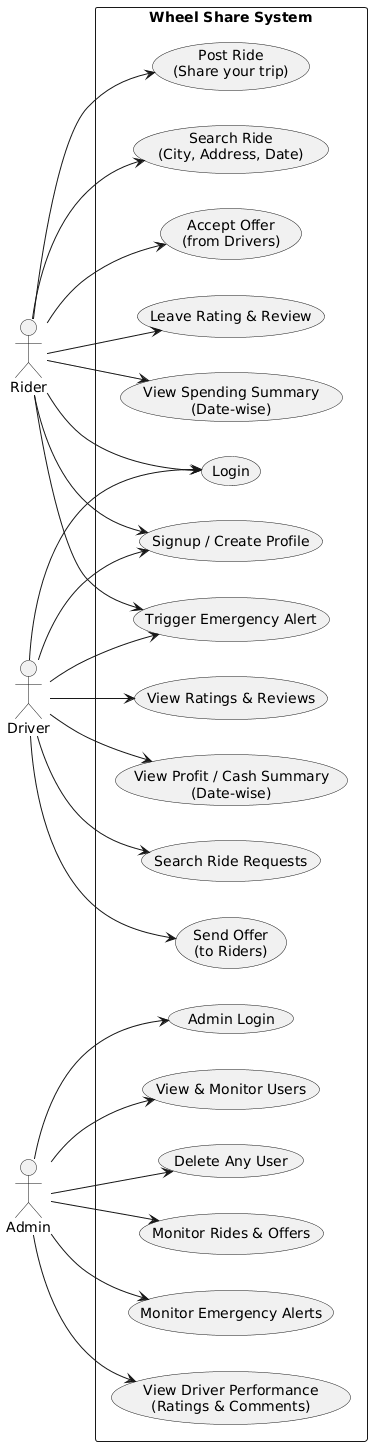
\includegraphics[height=0.95\textheight, keepaspectratio]{usecase_wheelshare.png}
    \caption{Use Case Diagram}
    \label{fig:usecase-diagram}
\end{figure}

\section{Use Case Specifications}


\subsection{Use Case: User Login}

\begin{table}[H]
\centering

\label{tab:usecase-login}
\renewcommand{\arraystretch}{1.2}
\begin{tabular}{|>{\bfseries}l|p{10cm}|}
\hline
Use Case ID & UC001 \\ \hline
Actor & User, Driver, Admin \\ \hline
Trigger & User submits credentials. \\ \hline
Pre-Condition & Registered user account exists. \\ \hline
Post-Condition & User successfully authenticated. \\ \hline
Flow &
1. User opens the app. \newline
2. User selects the login option. \newline
3. User enters login details. \newline
4. System verifies the account. \newline
5. User completes the login process. \\ \hline
\end{tabular}
\caption{Use Case for User Login}
\end{table}

\noindent
\textbf{Description:} This use case describes the authentication process where users log in using valid credentials and are redirected to their respective dashboards.

\subsection{Use Case: Sign Up}

\begin{table}[H]
\centering

\label{tab:usecase-signup}
\renewcommand{\arraystretch}{1.2}
\begin{tabular}{|>{\bfseries}l|p{10cm}|}
\hline
Use Case ID & UC002 \\ \hline
Actor & Rider, Driver \\ \hline
Trigger & User opens the sign-up page. \\ \hline
Pre-Condition & Email is not already registered. \\ \hline
Post-Condition & Account is created and profile is saved. \\ \hline
Flow &
1. User enters personal details. \newline
2. User verifies email. \newline
3. User creates profile. \newline
4. User logs into the system. \\ \hline
\end{tabular}
\caption{Use Case for Sign Up}
\end{table}

\noindent
\textbf{Description:} This use case explains the registration process for new users to create an account and access the system.


\subsection{Use Case: Post Ride}

\begin{table}[H]
\centering

\label{tab:usecase-postride}
\renewcommand{\arraystretch}{1.2}
\begin{tabular}{|>{\bfseries}l|p{10cm}|}
\hline
Use Case ID & UC003 \\ \hline
Actor & Rider \\ \hline
Pre-Condition & Rider is logged into the system. \\ \hline
Post-Condition & Ride is stored and visible to drivers. \\ \hline
Flow &
1. Rider enters ride details. \newline
2. Rider submits the ride. \newline
3. Ride becomes available for joining. \\ \hline
\end{tabular}
\caption{Use Case for Post Ride}
\end{table}

\noindent
\textbf{Description:} This use case allows riders to post ride details so that drivers can view and join the ride.

\subsection{Use Case: Search Ride / Send Offer / Accept Offer}

\begin{table}[H]
\centering

\label{tab:usecase-ridesearch}
\renewcommand{\arraystretch}{1.2}
\begin{tabular}{|>{\bfseries}l|p{10cm}|}
\hline
Use Case ID & UC004 \\ \hline
Actors & Rider, Driver \\ \hline
Pre-Condition & User is logged in and rides are available. \\ \hline
Post-Condition & Ride is confirmed if offer is accepted. \\ \hline
Flow &
1. Driver searches available rides. \newline
2. Driver sends an offer. \newline
3. Rider accepts or rejects the offer. \\ \hline
\end{tabular}
\caption{Use Case for Ride Search and Offer Management}
\end{table}

\noindent
\textbf{Description:} This use case defines the interaction between riders and drivers for ride matching and confirmation.




\subsection{Use Case: Ratings and Reviews}

\begin{table}[H]
\centering

\label{tab:usecase-ratings}
\renewcommand{\arraystretch}{1.2}
\begin{tabular}{|>{\bfseries}l|p{10cm}|}
\hline
Use Case ID & UC005 \\ \hline
Actors & Rider, Driver \\ \hline
Trigger & Completion of a ride. \\ \hline
Pre-Condition & Ride must be completed successfully. \\ \hline
Post-Condition & Feedback is saved and displayed. \\ \hline
Flow &
1. User selects completed ride. \newline
2. User submits rating and review. \\ \hline
\end{tabular}
\caption{Use Case for Ratings and Reviews}
\end{table}

\noindent
\textbf{Description:} This use case allows users to rate each other and provide feedback after a completed ride.


\subsection{Use Case: Spending Summary}

\begin{table}[H]
\centering

\label{tab:usecase-summary}
\renewcommand{\arraystretch}{1.2}
\begin{tabular}{|>{\bfseries}l|p{10cm}|}
\hline
Use Case ID & UC006 \\ \hline
Actors & Rider, Driver \\ \hline
Trigger & User opens summary module. \\ \hline
Pre-Condition & Ride history exists. \\ \hline
Post-Condition & Summary is displayed. \\ \hline
Flow &
1. User selects date range. \newline
2. System displays earnings or spending. \\ \hline
\end{tabular}
\caption{Use Case for Spending Summary}
\end{table}

\noindent
\textbf{Description:} This use case enables users to track their earnings or spending within a selected time period.

\subsection{Use Case: Emergency Feature}

\begin{table}[H]
\centering

\label{tab:usecase-emergency}
\renewcommand{\arraystretch}{1.2}
\begin{tabular}{|>{\bfseries}l|p{10cm}|}
\hline
Use Case ID & UC007 \\ \hline
Actors & Rider, Driver, Admin \\ \hline
Trigger & User presses emergency button. \\ \hline
Pre-Condition & Ride is ongoing. \\ \hline
Post-Condition & Emergency alert is logged. \\ \hline
Flow &
1. User triggers alert. \newline
2. System notifies admin. \\ \hline
\end{tabular}
\caption{Use Case for Emergency Feature}
\end{table}

\noindent
\textbf{Description:} This use case ensures user safety by allowing emergency alerts during an active ride.


\subsection{Use Case: Admin Monitoring}

\begin{table}[H]
\centering

\label{tab:usecase-admin}
\renewcommand{\arraystretch}{1.2}
\begin{tabular}{|>{\bfseries}l|p{10cm}|}
\hline
Use Case ID & UC008 \\ \hline
Actors & Admin \\ \hline
Trigger & Admin logs into the system. \\ \hline
Pre-Condition & Admin authentication successful. \\ \hline
Post-Condition & System activities are monitored. \\ \hline
Flow &
1. Admin monitors users and rides. \newline
2. Admin manages emergency alerts. \\ \hline
\end{tabular}
\caption{Use Case for Admin Monitoring}
\end{table}

\noindent
\textbf{Description:} This use case allows the administrator to monitor system activities and manage users.


\section{Project Feasibility}
The Wheel Share solution is most likely to be realized since it is based on open source technologies that prove to be inexpensive and have a scalable architecture. Flutter and Supabase can be used to dramatically decrease development cost and provide high-performing and cross-platform compatibility. The modularity of the application helps to make the future development of the app easier and manageable in terms of maintenance. Its friendly interface, which is based on the secure backend management, makes it applicable in the real world application. Besides, it covers the issues of affordability, convenience and safety thus finding its place in the area of community ride-sharing which makes the system sustainable in terms of urban mobility. 

